\subsubsection{Image Buffers}
\label{subsubsec:buffers}
\todo[inline]{Citations}

Two different buffers with the same buffer size (\texttt{BS}) are used.
A Baumer image buffer to receive the images and an OpenCV matrix cirucular buffer to manipulate and save the images.

% Buffer handling by Baumer => large buffer sizes (here not a problem), could be handled by ourselves!
  % handle this by ourselves on the Ultra96 board, due to memory size constrains
\paragraph{Baumer Image Buffer}
The received images are stored in Baumer \texttt{BGAPI2::Buffer} objects.
These are instantiated with the default constructor \texttt{BGAPI2::Buffer::Buffer()}, which allocates enough memory for the maximum payload of the camera.
In this case the maximum payload of the industrial camera is determined by the \texttt{BGR8} pixel format.
% Table \ref{tab:buffer_memory_utilization} shows that the memory utilization for the Baumer \texttt{BayerRG8} pixel format is only \SI{33}{\percent}.
As a result of this, the memory utilization for the Baumer \texttt{BayerRG8} pixel format is only \SI{33}{\percent}.
Table \ref{tab:buffer_memory_utilization} shows the required memory as well as the memory utilization for the two pixel formats \texttt{BayerRG8} and \texttt{BGR8}.

% The necessary memory for the Baumer \texttt{BayerRG8} pixel format could be allocated manually and then passed to the constructor.
% For convenience, the image buffer is hadeled by the Baumer GAPI.
It is possible to get \SI{100}{\percent} memory utilization with the Baumer \texttt{BayerRG8} pixel format.
The necessary memory could be allocated manually and then passed to the constructor.
However, the software is not designed to run on an embedded system but on a computer.
Every modern computer should have the required resources to run the program.
% https://www.baumer.com/ch/en/product-overview/industrial-cameras-image-processing/software/baumer-gapi-sdk/c/14174

% The function BGAPI2::Buffer::Buffer() creates a buffer the size of the maximum
% payload of the camera that is connected. This enables switching between the pixel formats and various image details without the need for size checking or recreating the buffer,
% since all formats will fit within the buffer. 
% If a lot of buffer space is required for small image details (ROI); this creates a high memory
% requirement, although only a small portion of this is actually used.

% Alternatively the user may allocate the buffer memory on its own using the function BGAPI2::Buffer:: Buffer( void *pUserBuffer, bo_uint64
% uUserBufferSize, void *pUserObj);
% The responsibility to release the allocated memory then remains with the user.
% The buffer size can be adjusted to the required payload size. This enables many buffers
% with small image details (ROI).
% The payload size for the current camera parameter settings (ROI or pixel format) can
% be determined using the query pDevice->GetRemoteNode(„PayloadSize")-
% >GetInt().

\begin{table}[h]
  \caption{Baumer image buffer memory utilization for the pixel formats \texttt{BayerRG8} and \texttt{BGR8}}
  \label{tab:buffer_memory_utilization}
  \centering
  \begin{tabular}{lll}
    \toprule
     & \textbf{\texttt{BayerRG8}} & \textbf{\texttt{BGR8}} \\
    \midrule
    \textbf{Bytes per pixel} & \SI{1}{B} & \SI{3}{B} \\
    \textbf{Pixel count} & \SI{1310720}{px} & \SI{1310720}{px} \\
    \textbf{Pixel bytes} & \SI{1310720}{B} & \SI{3932160}{B} \\
    \textbf{Buffer size} & \SI{3932160}{B} & \SI{3932160}{B} \\
    \textbf{Utilization} & \SI{33}{\percent} & \SI{100}{\percent} \\
    \bottomrule
  \end{tabular}
\end{table}



% --------------------------------
\paragraph{OpenCV Circular Buffer}
% opencv matrix circular buffer (same size as Baumer buffer but shallow [shallow-copy])
  % only pointer to the baumer pixel data
  % copying would require a lot of space and time (which is not much to play with), thus main reason time
% circular buffer graphic

OpenCV matrix \texttt{cv::Mat} objects are used to perform the necessary image manipulations (see section \ref{subsubsec:image_change_detection}).
The data pointer of the Baumer image buffer is used to create an OpenCV matrix as shown in appendix \ref{app:throw_detection} on line \ref{lst:ln:buffer}.
This way, the OpenCV matrix does not allocate memory for the matrix data and uses the specified data.
The reasons for only creating such a shallow copy are efficiency and memory space.
% https://docs.opencv.org/4.1.1/d3/d63/classcv_1_1Mat.html#a51615ebf17a64c968df0bf49b4de6a3a
% https://www.baumer.com/ch/en/service-support/know-how/technical-information-industrial-cameras/baumer-gapi-and-opencv/a/baumer-gapi-and-opencv

% Saving the images later on requires to keep track of past OpenCV matrices.
% In order to be able to save the images later, past OpenCV matrices must be kept track of.
In order to be able to save the images later, past OpenCV matrices must be available.
For this reason, an OpenCV matrix circular buffer is used to keep track of them.
The structure of the circular buffer is shown in figure \ref{fig:circular_buffer}.
The circular buffer size (\texttt{BS}) is the same as the Baumer image buffer size.
The elements of the circular buffer can be accessed through an index $I$.
This index $I$ depends on the frame id (\texttt{FID}) and is calculated using equation \ref{eq:indexing}.

\begin{equation}
  I \equiv \text{FID} \pmod{\text{BS}}
  \label{eq:indexing}
\end{equation}

\begin{figure}[h]
  \centering
  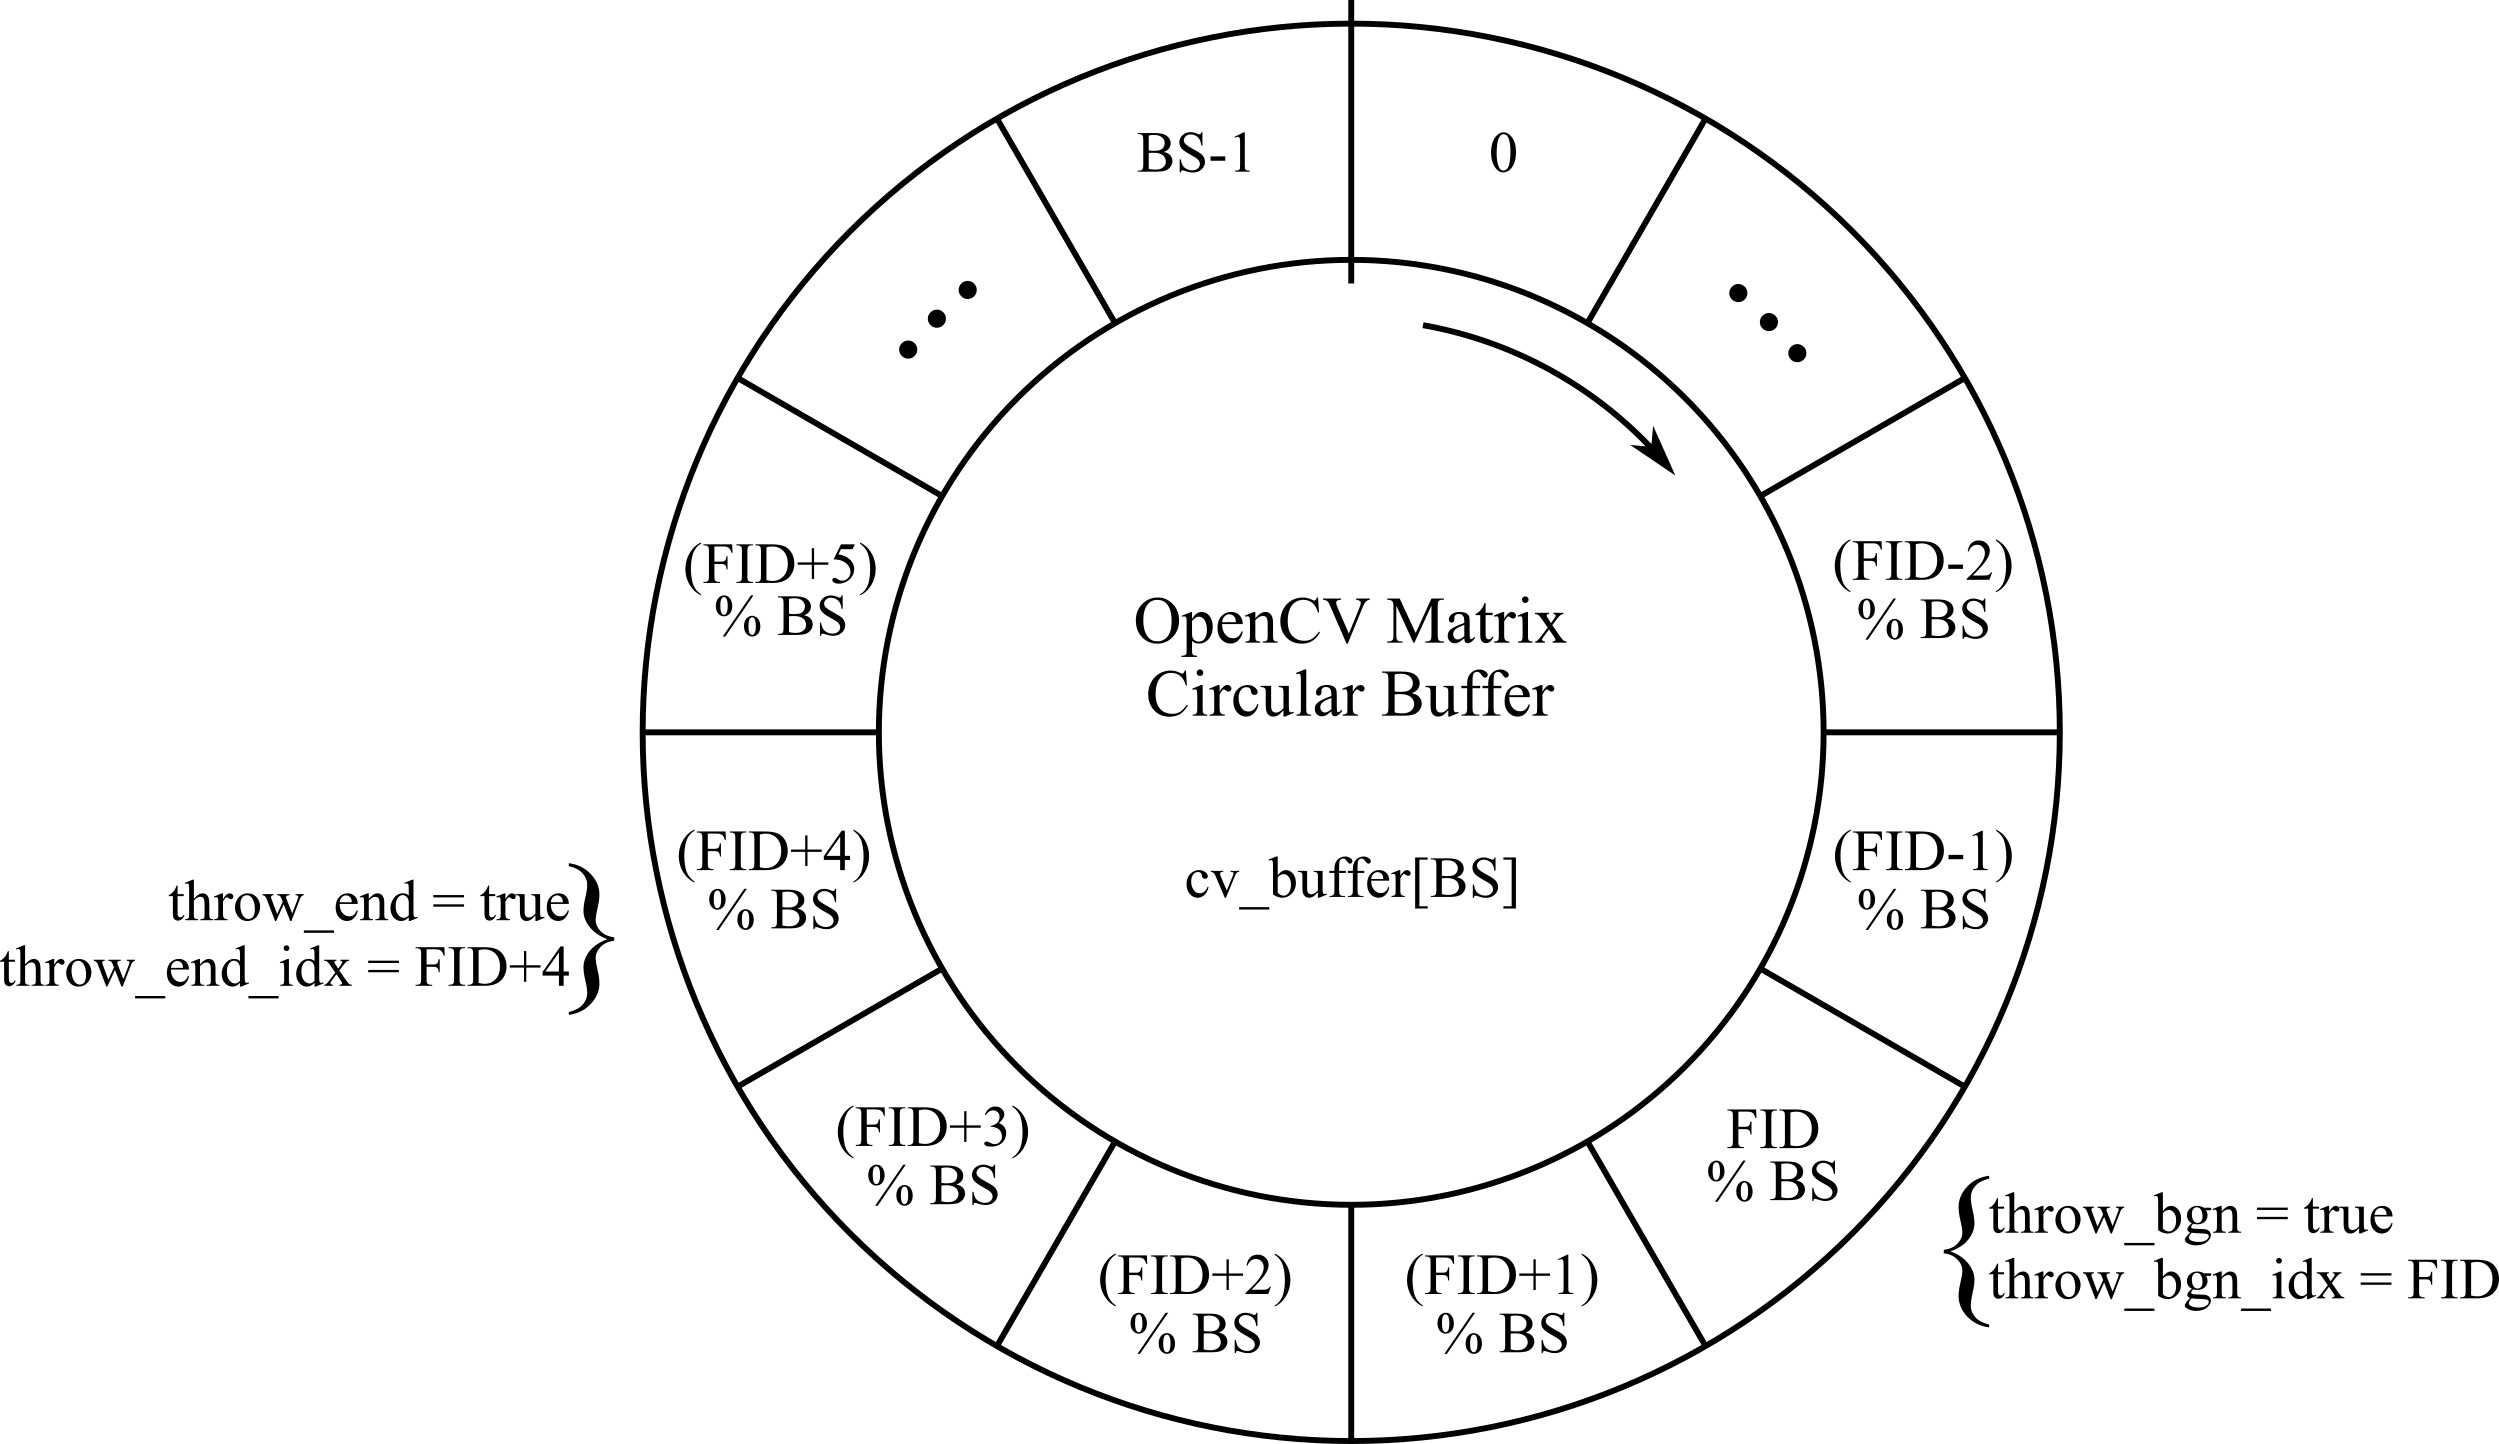
\includegraphics[width=0.9\textwidth]{buffer}
  \caption{OpenCV matrix circular buffer}
  \label{fig:circular_buffer}
\end{figure}

% \begin{lstlisting}[style=C++]
%   cv_buffer[frame_id % buff_size] = cv::Mat(height, width, CV_8UC1, (void *) pBufferFilled->GetMemPtr());
% \end{lstlisting}

% Coupled Buffers
% Since RAW formats often have to be converted into other target formats, such as BGR8 or
% BGR12, you can couple an external user buffer to this internal buffer, which then accepts
% the transformed data.
% Using pBuffer->GetMemPtr() accesses the RAW image and pBuffer
% ->GetUserObj() accesses the memory area in the user buffer. In the example, the
% external user buffer is of a size that equates to the target pixel format "BGR8", which
% requires 3 bytes per pixel.
